%%%%%%%%%%%%%%%%%%%%% appendix.tex %%%%%%%%%%%%%%%%%%%%%%%%%%%%%%%%%
%
% sample appendix
%
% Use this file as a template for your own input.
%
%%%%%%%%%%%%%%%%%%%%%%%% Springer-Verlag %%%%%%%%%%%%%%%%%%%%%%%%%%

\appendix

\begin{partbacktext}
\part{Appendix: Mathematical Foundations and Competition}\label{part:math}


The appendix includes contents that serves as the preliminary knowledge of the technical chapters, including probability theory and linear algebra. Only very basic contents are included, and the readers are referred to dedicated textbooks for more in-depth contents. 
Moreover, we also include some contents for probabilistic graphical model, in addition to the introductory content already provided in Chapter~\ref{chap:pgmfeature}. 
Finally, we also include a competition that is designed for a group of students to learn adversarial attack and training by competing with each other's solutions. 
\end{partbacktext}

%\newpage 
\chapter{Probability Theory}

\section{Random Variables}

In most of our contexts, a random variable is a function that assigns probability values to each of an experiment's (or an event's) outcomes. Intuitively, a random variable has a probability distribution, which represents the likelihood that any of the possible values would occur.

\begin{example}\label{example:foundationsgrades}
We have a population of students, such that we want to reason about their grades. In this case, we have 
\begin{itemize}
    \item a random variable $Grade$, with the set of possible values $V(Grade)=\{ A, B, C \}$, and 
    \item a function $P(Grade)$, which associates a probability with each outcome. 
\end{itemize}
\end{example}



Given $P(X)$ is a probability distribution, we have 
\begin{equation}
    \sum_{x\in V(X)} P(x) = 1
\end{equation}
and we may call $P(X)$ the marginal distribution of $X$, as opposed to the joint and conditional distributions. We will explain these concepts in detail later.  

A probability distribution $P(X)$ is a multi-nominal distribution if there are multiple values for the random variable $X$, i.e., $|V(X)|>1$. Moreover, if $V(X)=\{false,true\}$ then $P(X)$ is a Bernoulli distribution. Besides, $P(X)$ can be continuous, such that it may take on an uncountable set of values. 

\begin{example}
The $Grade$ random variable in Example~\ref{example:foundationsgrades} has three possible values and therefore it is associated with a multi-nominal distribution. Also, for a coin tossing example with a single coin that may be either head or tail, the random variable $Coin$ is associated with a Bernoulli distribution. Moreover, a real-valued random variable is continuous, even if it only takes values from a real interval. 
\end{example}


A random variable can also be multi-dimensional. 

\begin{example}
For the \textbf{iris} example as in Example~\ref{example:iris}, the data instance can be seen as a 4-dimensional continuous variable $X$, such that it has an underlying data distribution and the dataset is sampled from the data distribution. The label $Y$ can be seen as another random variable.    
\end{example}

%Such a distribution is also referred to as a multi-nomial distribution as there are multiple values for the random variable $X$. If 

%Also, 

\section{Joint and Conditional Distributions}

A marginal probability is the probability of an event $X$ occurring, i.e., $P(X)$. It may be thought of as an unconditional probability, as it is not conditioned on any other event.

\begin{example}
Assume that we randomly draw a card from a standard deck of playing cards. Let $C$ be the random variable, representing the color of the card drawn. Then, the probability that the card drawn is red is $P(C = red) = 0.5$, or simply $P(red) = 0.5$ if the random variable $C$ is clear from the context.
\end{example}

\begin{example}
Given a standard deck of playing cards, the probability that a card drawn is a 4 is $P(four)=1/13$.
\end{example}
%• Another example: 

\subsection*{Joint probability $P(X,Y)$} 
is the probability of event $X$ and event $Y$ occurring. It is a statistical measure that calculates the likelihood of two events occurring at the same time. %It is the probability of the intersection of two or more events. The probability of the intersection of $A$ and $B$ may be written $P(A \cap B)$.

\begin{example}
Given a standard deck of playing cards, the probability that a card is a four and red, i.e., $P(four, red) = 2/52=1/26$. Note: there are two red fours in a deck of 52, the 4 of hearts and the 4 of diamonds.
\end{example}

The joint probability can be generalised to work with more than two events. 


\subsection*{Conditional probability $P(X|Y)$}
 is the probability of event $X$ occurring, given that event $Y$ has already occurred.

\begin{example}
Given a standard deck of playing cards, if we know that you have drawn a red card, what is the probability that it is a four? The answer is  $P(four|red)=2/26=1/13$, i.e., out of the 26 red cards (given a red card), there are two fours, so $2/26=1/13$.
\end{example}

\section{Independence and Conditional Independence}\label{sec:indepandcondindep}

Without loss of generality, we assume that for the remaining of this section, all random variables are Boolean. 
Given two Boolean random variables $X$ and $Y$, we expect that, in general, $P(X|Y)$ is different from $P(X)$, i.e., the fact that $Y$ is true may  change our probability over $X$.  

\subsection*{Independence}

Sometimes an equality can occur, i.e, $P(X|Y)=P(X)$.  
 i.e., learning that $Y$ occurs does not change our probability of $X$. In this case, we say event $X$ is independent of event $Y$, denoted as %
 \begin{equation}
     X \bot Y
 \end{equation}
%
A distribution $P$ satisfies $X \bot Y$ if and only if $P(X,Y)=P(X)P(Y)$. %A more common situation is when two events are independent given an additional event 


\begin{example}\label{example:independenceexample}
Consider the joint probability table as shown in Table~\ref{tab:simpleJointProbability}. 
\begin{table}[!htbp]
    \centering
    \begin{tabular}{|c|c|c|}
    \hline
        X & Y & P(X,Y)  \\
        \hline
        $0$  &  $0$ & 0.08 \\
        $0$  &  $1$ & 0.32 \\
        $1$  &  $0$ & 0.12 \\
        $1$  &  $1$ & 0.48 \\
        \hline
    \end{tabular}
    \caption{A simple two variable joint distribution}
    \label{tab:simpleJointProbability}
\end{table}

First of all, we note that 
\begin{equation}
    \begin{array}{lcl}
        P(X=0) & = & 0.32+0.8 = 0.4 \\
        P(X=1) & = & 0.6 \\
        P(Y=0) & = & 0.08+0.12 = 0.2 \\
        P(Y=1) & = & 0.8 \\
    \end{array}
\end{equation}
Then, we notice that 
\begin{equation}
    \begin{array}{lclclcl}
      0.08 & = &  P(X=0,Y=0) & = & P(X=0)*P(Y=0) & = & 0.4 * 0.2 \\
      0.32 & = &  P(X=0,Y=1) & = & P(X=0)*P(Y=1) & = & 0.4 * 0.8 \\
      0.12 & = &  P(X=1,Y=0) & = & P(X=1)*P(Y=0) & = & 0.6 * 0.2 \\
      0.48 & = &  P(X=1,Y=1) & = & P(X=1)*P(Y=1) & = & 0.6 * 0.8 \\
    \end{array}
\end{equation}
that is, 
\begin{equation}
    P(X,Y) = P(X) * P(Y)
\end{equation}
which suggests that $X$ and $Y$ are independent.
\end{example}

\begin{example}\label{example:noindependence}
On the other hand, for the following Table~\ref{tab:simpleJointProbability2}, the two variables $X$ and $Y$ are not independent.  

\begin{table}[!htbp]
    \centering
    \begin{tabular}{|c|c|c|}
    \hline
        X & Y & P(X,Y)  \\
        \hline
        $0$  &  $0$ & 0.10 \\
        $0$  &  $1$ & 0.16 \\
        $1$  &  $0$ & 0.64 \\
        $1$  &  $1$ & 0.10 \\
        \hline
    \end{tabular}
    \caption{Another simple two variable joint distribution}
    \label{tab:simpleJointProbability2}
\end{table}
\end{example}


\subsection*{Conditional independence}


While independence is a useful property, we do not often encounter two independent events.  
A more common situation is when two events $X$ and $Y$ are independent given an additional event $Z$, denoted as 
 \begin{equation}
     X \bot Y | Z
 \end{equation}
A distribution $P$ satisfies $X \bot Y | Z$ if and only if $P(X,Y | Z)=P(X | Z)P(Y | Z)$. 

Note that, similar calculation as in Examples~\ref{example:independenceexample} and \ref{example:noindependence} can be done to work with conditional independence, with the only changes on replacing the computation of marginal probabilities $P(X)$ and $P(Y)$ with the computation of conditional probabilities $P(X | Z)$ and $P(Y | Z)$.


\section{Querying Joint Probability Distributions}

A joint distribution $P(X_1,...,X_n)$ contains an exponential number $2^n$ of real probability values and it can be hard to make sense of them. It is desirable that we are able to infer useful information by making queries. 
%
In the following, we introduce a few categories of queries. 

\subsection*{Probability queries} 

are to compute distribution of a subset of random variables, given  evidence (i.e., the values) of another subset of random variables. Formally, it is to compute
\begin{equation}
    P(X_{i1},...,X_{ik}| X_{j1}=x_{j1},...,X_{jl}=x_{jl})
\end{equation}
where $x_{j1},...,x_{jl}$ are evidence for the random variables $X_{j1},...,X_{jl}$, respectively. Moreover, we have  $\{X_{i1},...,X_{ik}\}\cup \{X_{j1},...,X_{jl}\}\subseteq \{X_1,...,X_n\}$ and $\{X_{i1},...,X_{ik}\}\cap  \{X_{j1},...,X_{jl}\} = \emptyset$. 

\subsection*{Maximum a posteriori (MAP) queries}

In addition to probability queries which concern the (conditional) probability of the occurrence of events, we may be interested in MAP-style queries, which is to find a joint assignment to some subset of variables that has the highest probability. For simplicity, we let $\{X_1,...,X_k\}, \{X_{k+1},...,X_l\}, \{X_{l+1},...,X_n\}$ be three disjoint subsets of the random variables $\{X_1,...,X_n\}$. Then, the MAP query is of the form  
\begin{equation}
\begin{array}{rl}
     &  MAP(X_1,...,X_k|X_{l+1},...,X_n) \\
   =  & \displaystyle\argmax_{x_1,...,x_k} \sum_{x_{k+1},...,x_{l}}P(X_{1}=x_1,...,X_{l}=x_l| X_{l+1}=x_{l+1},...,X_{n}=x_{n})
\end{array}
\end{equation}
Intuitively, we have the evidence for variables $\{X_{l+1},...,X_n\}$, and intend to find the joint assignment for $\{X_1,...,X_k\}$. Because we do not have information about $\{X_{k+1},...,X_l\}$, we marginalise them. 

\begin{example}
Consider a probability table for variable $X_1$ as in Table~\ref{tab:tableforx1}.  
\begin{table}[!htbp]
    \centering
    \begin{tabular}{|c|c|}
    \hline
        $X_1 = 0$ & $X_1 = 1$ \\
        \hline
        0.4 & 0.6\\
        \hline
    \end{tabular}
    \caption{Probability table for $X_1$}
    \label{tab:tableforx1}
\end{table}

Then, we have $MAP(X_1)=1$. 
\end{example}

\begin{example}
Consider a joint probability table for variables $X_1$ and $X_2$ as in Table~\ref{tab:tableforx1x2}. 
\begin{table}[!htbp]
    \centering
    \begin{tabular}{|c|c|c|}
    \hline
        $X_1$ & $X_2$ & $P(X_1,X_2)$ \\
        \hline
        0 & 0 & 0.04\\
        0 & 1 & 0.36 \\
        1 & 0 & 0.3 \\
        1 & 1 & 0.3\\
        \hline
    \end{tabular}
    \caption{Joint probability table for $X_1$ and $X_2$}
    \label{tab:tableforx1x2}
\end{table}

Then, we have $MAP(X_2)=1$. 
\end{example}

%Maximum a posteriori probability 
%Also called MPE (Most Probable Explanation) 
%What is 
%Marginal MAP Queries




\newpage
\chapter{Linear algebra}


\section{Scalars, Vectors, Matrices, Tensors} 

\subsection*{Scalar} 

A scalar is a single number. It is represented in lower-case italic, such as $x$. 

\begin{example}
We can use $x\in\real$, a real-valued scalar, to define the slope of the line. Moreover, we can use $x\in \nat$, a natural number scalar, to define  the number of units. 

\end{example}

\subsection*{Vector}  A vector is an array of numbers arranged in order. Each number in a vector is identified with an index. Vectors are represented as lower-case bold, such as $\textbf{x}$. If $x$ is $n$-dimensional and each element of $\textbf{x}$ is a real number, we write $\textbf{x}\in \real^n$. 

Geometrically, we think of vectors as points in space such that each element of a vector gives coordinate along an axis. This is the same as we consider a data instance -- usually represented as a vector -- as a point in high-dimensional space. 


\subsection*{Matrix} A matrix is a 2-D array of numbers, such that each element is identified by two indices. Matrices are represented as bold typeface $\textbf{A}$. We usually identify each element of $\textbf{A}$ with the subscripts, i.e., use $\textbf{A}_{i,j}$ to denote the element on the $i$-th row and $j$-th column. We may also write $\textbf{A}[i:]$ for the $i$-th row of $\textbf{A}$ and $\textbf{A}[:j]$ the $j$-th column of $\textbf{A}$. Similar as the vectors, we may write $\textbf{A}\in\real^{m\times n}$ if $\textbf{A}$ has $m$ rows and $n$ columns and each element is a real number. 
 



\subsection*{Tensor} It is very likely in a machine learning context that, we may need an array with more than two axes. We call a multi-dimensional array arranged on a regular grid with variable number of axes as a tensor.  Tensors are also represented as bold typeface $\textbf{A}$, and we may use the subscripts to identify its element, for example  $\textbf{A}_{i,j,k}$ to denote the element in a three-dimensional tensor. We remark that, a tensor may include more involved properties that a multi-dimensional array does not have, but we omit the details for the simplicity of the explanations. 



\section{Matrix Operations}

We briefly review a few frequently used matrix operations. 

\subsection*{Transpose of a Matrix }

The transpose of a matrix is an operator which flips a matrix over its diagonal. Given a matrix $\textbf{A}$, we define its transpose $\textbf{A}$ as that 
\begin{equation}
    \textbf{A}^T_{ij} = \textbf{A}_{ji} \text{ for all } i,j 
\end{equation}


\subsection*{Linear Transformation}

A linear transformation is a function from one vector space to another that respects the underlying (linear) structure of each vector space.  Linear transformations can be represented by matrices. If $T$ is a linear transformation mapping from $\real^n$ to $\real^m$, and $\textbf{x}$ is a column vector with $n$ entries, then 
\begin{equation}
    T(\textbf{x}) = \textbf{A}\textbf{x}
\end{equation}
for some $m\times n$ matrix $\textbf{A}$. Also, $\textbf{A}$ is called transformation matrix of $T$. 

\subsection*{Identity Matrix}

The identity matrix of size $n$ is the $n \times n$ square matrix with ones on the diagonal and zeros elsewhere. We use $\textbf{I}$ to denote an identity matrix. 

\subsection*{Matrix Inverse }

An $n\times n$ matrix $\textbf{A}$ is invertible if there exists another $n\times n$ matrix $\textbf{A}$ such that 
\begin{equation}
    \textbf{A}\textbf{B} = \textbf{B} \textbf{A} = \textbf{I}
\end{equation}
We write $\textbf{B}$ as the inverse of $\textbf{A}$, denoted as  $\textbf{A}^{-1}=\textbf{B}$, 

%\subsection*{Solving Simultaneous equations }

\section{Norms}\label{sec:norms}

Usually, a distance function is employed to compare data instances. Ideally, such a distance should reflect perceptual similarity between data instances, comparable to e.g., human perception for image classification networks. A distance metric should satisfy a few axioms which are usually needed for defining a metric space: 
\begin{itemize}
\item $||\textbf{x}||\geq 0$ (non-negativity),
\item $||\textbf{x}-\textbf{y}||=0$ implies that $\textbf{x} = \textbf{y}$ (identity of indiscernibles),
\item $||\textbf{x}-\textbf{y}|| = ||\textbf{y}-\textbf{x}||$ (symmetry),
\item $||\textbf{x}-\textbf{y}||+||\textbf{y}-\textbf{z}|| \geq ||\textbf{x}-\textbf{z}||$ (triangle inequality).
\end{itemize}

In practise, $L_p$-norm distances are used, including

\begin{itemize}
    \item $L_1$ (Manhattan distance): \begin{equation}
        ||\textbf{x}||_1 = \sum_{i=1}^{n} |x_i|
    \end{equation}
    \item $L_2$ (Euclidean distance):
    \begin{equation}||\textbf{x}||_2 = \sqrt{\sum_{i=1}^{n} x_i^2}\end{equation}
    \item $L_\infty$ (Chebyshev distance): \begin{equation}||\textbf{x}||_\infty  = \max_{i} |x_i|\end{equation}
\end{itemize}
Moreover, we also consider $L_0$-norm as $||\textbf{x}||_0 = |\{x_i~|~x_i\neq 0, i = 1..n\}|$, i.e., the number of non-zero elements. Note that, $L_0$-norm does not satisfy the triangle inequality. 
In addition to these, there exist other distance metrics such as Fréchet Inception Distance \cite{10.5555/3295222.3295408}. In addition, Frobenius norm of a matrix is represented by $||\cdot||_{\mathrm{Fr}}$.

Given a data instance $x$ and a distance metric $L_p$, the \emph{neighbourhood} of $\textbf{x}$ is defined as follows.
\begin{definition}[d-Neighbourhood]\label{def:inputregion}
Given a data instance $\textbf{x}$, a distance function $L_p$, and a distance $d$, we define 
the \emph{d-neighbourhood} $\eta(\textbf{x},L_p,d)$ of $\textbf{x}$ w.r.t. $L_p$ as 
\begin{equation}
\eta(\textbf{x},L_p,d)=\{\hat{\textbf{x}} ~|~ \distance{\hat{\textbf{x}}-\textbf{x}}{p} \leq d\},
\end{equation}
the set of data instances whose distance to $\textbf{x}$ is no greater than $d$ with respect to $L_p$.  
\end{definition}


\section{Variance, Covariance, and Covariance Matrix}\label{sec:variance}

\subsection*{Variance} measures the variation of a single random variable. Formally, 
\begin{equation}
    Var(X) = \mathbb{E}[(X-\overline{X})^2]
\end{equation}
where $\displaystyle\overline{X}=\mathbb{E}[X]$ is the mean. If we are working with a finite set $D$ of data samples, we have 
% and 
\begin{equation}
  \overline{X}=\frac{1}{|D|}\sum_{\textbf{x}\in D}\textbf{x} \hspace{2cm} Var(X) = \frac{1}{|D|} \sum_{\textbf{x}\in D}(\textbf{x} - \bar{X})^2
\end{equation}
where $|D|$ denotes the number of samples in $D$. 
%

\subsection*{Covariance}, based on variance, measures how much two random variables vary together. Formally, 
\begin{equation}
    Cov(X,Y) = \mathbb{E}[(X-\mathbb{E}[X])(Y-\mathbb{E}[Y])]
\end{equation}
If working with a dataset $D$ of $(\textbf{x},\textbf{y})$ pairs, it is 
\begin{equation}
    Cov(X,Y) = \frac{1}{|D|} \sum_{(\textbf{x},\textbf{y})\in D}(\textbf{x} - \bar{X})(\textbf{y}- \bar{Y})
\end{equation}

\subsection*{Covariance Matrix} Generalising the above, consider a column vector $\textbf{X} = (X_1,...,X_n)^T$ of random variables, we can have the covariance matrix as follows: 
\begin{equation}
    \textbf{K}= \begin{bmatrix}
     Cov(X_1,X_1)       & Cov(X_1,X_2) & Cov(X_1,X_3) & \dots & Cov(X_1,X_n) \\
    Cov(X_2,X_1)       & Cov(X_2,X_2) & Cov(X_2,X_3) & \dots & Cov(X_2,X_n) \\
    \hdotsfor{5} \\
    Cov(X_n,X_1)       & Cov(X_n,X_2) & Cov(X_n,X_3) & \dots & Cov(X_n,X_n)
\end{bmatrix}
\end{equation}





%\part{Competitions}\label{part:competitions}

%\begin{partbacktext}
\chapter{Probabilistic Graph Models}\label{chap:pgm}
%\noindent Use the template \emph{part.tex} together with the document class SVMono (monograph-type books) or SVMult (edited books) to style your part title page and, if desired, a short introductory text (maximum one page) on its verso page.

%\end{partbacktext}
%\chapter{Probabilistic Graph Models for Feature Robustness}\label{chap:pgm}




%\newpage
\section{I-Maps}\label{sec:i-map}

This section studies the conditional independences in $G$. 

\subsection{Naive Bayes and Joint Probability}

First of all, we explain the difference between usual classification and Naive Bayes classifier. As shown in Figure~\ref{fig:naiveBayesPGM}, usual classification can be represented as a graphical model $G$ where the class label $Y$ receives incoming connections from the feature variables $X_1,...,X_n$. Therefore, $Y$ has a conditional probabilistic table $P(Y|X_1,...,X_n)$ and the feature variables $X_i$ has a marginal probability table $P(X_i)$. 
\begin{figure}[!htbp]
    \centering
    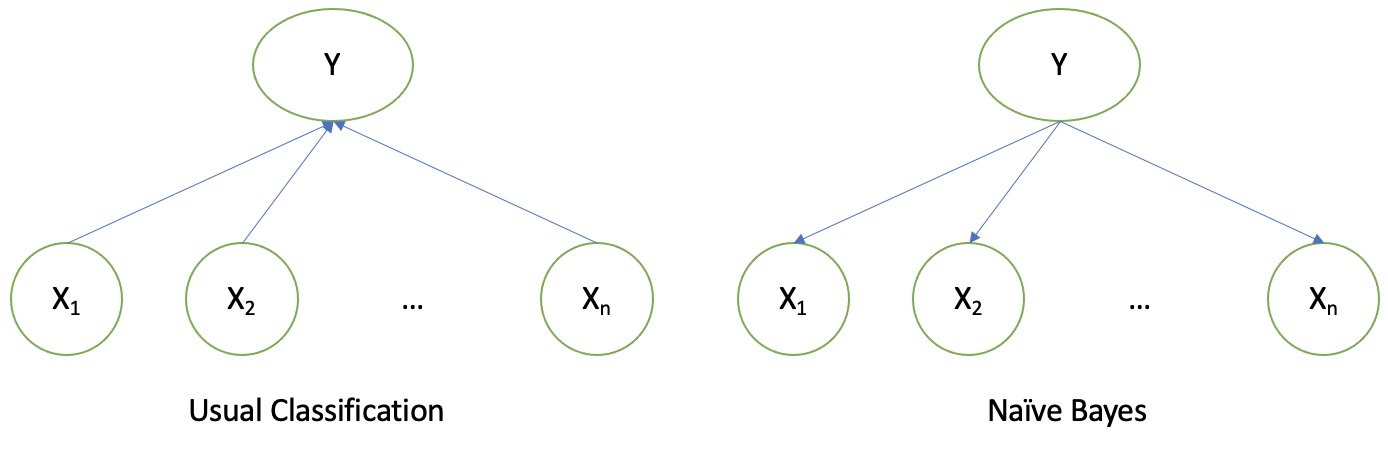
\includegraphics[width=0.9\textwidth]{images/graphical models/NaiveBayesPGM2.png}
    \caption{Naive Bayes as a probabilistic graphical model}
    \label{fig:naiveBayesPGM}
\end{figure}
However, for Naive Bayes classifier, it can be represented as another graphical model $G'$ where the label $Y$ has outgoing arrows to the feature variables $X_1,...,X_n$. Therefore, each feature variable $X_i$ has a conditional probability table $P(X_i|Y)$ and the class label has a marginal probability table $P(Y)$. As we explained earlier, for naive Bayes, we have 
%Intuitively, it says that, the random variable $Y$ conditionally depends on the other variables $X_1,...,X_n$, and once $Y$ is observed, $X_1,...,X_n$ are conditionally independent. We will explain this intuition later, and here we are interested to 
\begin{equation}
    P(X_1,...,X_n,Y)= P(Y)\prod_{i\in \{1..n\}}P(X_i|Y)
\end{equation}
That is, the joint probability is the product of probability tables for the nodes on the graph. Generalising the case for Naive Bayes classifier,  we conjecture that for 
 each probabilistic graphical model $G=({\cal V},{\cal E},P)$ represent the joint probability distribution between random variables, we may have  
\begin{equation}\label{equ:pajoint}
    P({\cal V})= \prod_{V\in {\cal V}}P(V|Pa(V))
\end{equation}
where $Pa(V)$ is the set of parent nodes of node $V$. Note that, we let $P(V|\emptyset) = P(V)$ when the node $V$ does not have incoming edges. 

\subsection{Independencies in a Distribution}\label{sec:distributionalindependencies}

Before proceeding to the conditional probabilities in $G$, we may need to know how to find conditional independencies from a joint probability. For this, Section~\ref{sec:indepandcondindep} has presented a few examples on how to do the calculation. 



 
\subsection{Markov Assumption}

In addition to the notation 
%We write 
$Pa(X)$ for the set of parents of a node $X$, we need $NonDesc(X)$ for the set of non-descendents of $X$. We have that 
\begin{tcolorbox}
each random variable $X$ is independent of its non-descendents, given its parents, i.e.,
\begin{equation}
    X\bot NonDesc(X) | Pa(X)
\end{equation}
\end{tcolorbox}
Intuitively, parents of a variable shield it from probabilistic influence. Once values of parents are  known, no influence of ancestors can be made. On the other hand, information about descendants can change beliefs about a node . 

For the running example in Figure~\ref{fig:graphicalmodel}, we have the following local conditional independences that can be read directly from the graph: 
\begin{equation}
    \begin{array}{lcl}
        I(G) &  = \{ & (Fog\bot Detected, Radar, Away, Stopped | Camera),  \\
         & & (Camera \bot Radar, Away) , \\
         & & (Radar \bot Camera, Fog) , \\
         & & (Detected \bot Away, Fog | Camera, Radar) , \\
         & & (Away  \bot Camera, Fog, Detected | Radar) , \\
         & & (Stopped \bot Fog, Camera, Radar | Detected, Away) \} \\
    \end{array}
\end{equation}
Intuitively, to understand $(Fog\bot Detected, Radar, Away, Stopped | Camera)$, we note  that, once we are able to observe the camera's result, the weather conditions such as $Fog$ can be directly obtained and are independent from other random variables. Moreover, to understand $(Camera \bot Radar, Away)$, we note that camera's precision -- as a quality of hardware --  is absolutely independent of both radar's result and whether or not the pedestrian is away. Other (conditional) independencies can be explained in a similar way. 

We remark that, the conditional independencies obtained through this way are local ones, and do not necessarily include all conditional independencies that can be inferred from the graph. In Section~\ref{sec:d-sep}, we will introduce a comprehensive method -- d-separation -- that is able to infer all possible conditional independencies from a graph. 

\subsection{I-Map of Graph and Factorisation of Joint Distribution}

Let $G$ be a graph associated with a set of independencies $I(G)$, and $P$ a probability distribution with a set of independencies $I(P)$. Note that, $I(P)$ can be obtained by the way shown in Section~\ref{sec:distributionalindependencies}. Then, we define 

\begin{definition}
$G$ is an I-Map of $P$ if $I(G)\subseteq I(P)$. 
\end{definition}

By this definition, I-Map requires that a joint
distribution $P$ can have more independencies than the graph $G$, but 
graph $G$ cannot mislead by containing independencies that do not exist in $P$. 

\begin{example}
Consider the joint probability table $P$ as in Table~\ref{tab:simpleJointProbability}, and the  three graphs in Figure~\ref{fig:simpleGs}. 
\begin{figure}[!htbp]
    \centering
    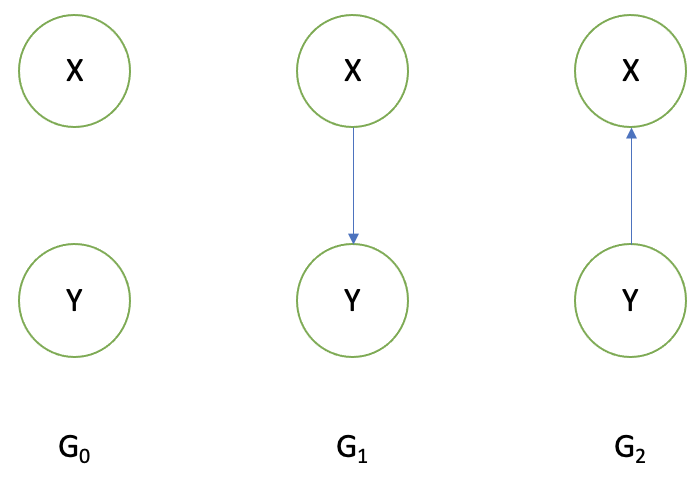
\includegraphics[width=0.4\textwidth]{images/graphical models/I-map/simpleGs.png}
    \caption{Three simple, two-node graphs}
    \label{fig:simpleGs}
\end{figure}
we note that $I(P)=\{X\bot Y\}$, $I(G_0)=\{X\bot Y\}$, and $I(G_1)=I(G_2)=\emptyset$. Therefore, all three graphs $G_0, G_1, G_2$ are I-maps of $P$. On the other hand, if consider  the joint probability table $P$ as in Table~\ref{tab:simpleJointProbability2}, we have that $I(P)=\emptyset$. Then, while $G_1$ and $ G_2$ are still I-maps of $P$, $G_0$ is not any more. 
\end{example}

In the following, we introduce the relationship between I-map and factorisation. Factorization is to write a mathematical object as a product of several, usually smaller or simpler, objects of the same kind. For example, in the Naive Bayes classifier, the joint distribution $P(X_1,...,X_n,Y)$ is rewritten as the production of $P(Y)$ and conditional probabilities $P(X_i|Y)$, where $P(Y)$ and $P(X_i|Y)$ are much smaller than $P(X_1,...,X_n,Y)$. For the graphical model in general, we have 

\begin{theorem}
If $G$ is an I-map of $P$, then 
\begin{equation}
    P(X_1,...,X_n) = \prod_{i=1}^n P(X_i|Pa(X_i))
\end{equation}
\end{theorem}
This justifies our conjecture at Equation (\ref{equ:pajoint}). 

\subsection{Perfect Map}

Similar as I-map, we may define D-map, which requires that $I(P)\subseteq I(G)$. The intersection of I-map and D-map leads to perfect map, which requires that the conditional independencies in $G$ and $P$. 
Interestingly, but not surprisingly, not all distributions $P$ over a given set of variables can be represented as a perfect map. 




%\newpage
\section{Reasoning Patterns}

As explained earlier, the construction of graphical models will enable our reasoning about a more complex relation between a set of random variables. In this section, we introduce a few typical reasoning patterns. 

\subsection{Causal Reasoning}

Causal reasoning considers how the changes of up-stream variables may affect the values of the down-stream variables. For our running example as in Figure~\ref{fig:cameratables}, it is for  an engineer to concern about how likely the car will stop given e.g., the quality of sensors (i.e., camera and/or radar). 

A typical process is to first compute a marginal probability such as 
\begin{equation}
    P(s_0) 
\end{equation}
which is the probability of the car does not stop. This can be computed by having 
\begin{equation}
\begin{array}{rl}
    P(s_0) = & \displaystyle\sum_{C,R,F,D,A} P(C,R,F,D,A,S=s_0) \\
    = & \displaystyle\sum_{i=0}^1\sum_{j=0}^1\sum_{k=0}^1\sum_{l=0}^1\sum_{m=0}^1 P(C=c_i,R=r_j,F=f_k,D=d_l,A=a_m,S=s_0)\\
    \approx & 0.62\\
\end{array}
\end{equation}
Then, we may consider a conditional probability such as 
\begin{equation}
    P(s_0|c_1) = \frac{P(s_0,c_1)}{P(c_1)} \approx 0.51
\end{equation}
which says that if we know that the camera captured the pedestrian, the probability of not stopped decreased to 0.51. Similarly, if  consider radar,  we have 
\begin{equation}
    P(s_0|r_1) = \frac{P(s_0,c_1)}{P(r_1)} \approx 0.44
\end{equation}

If both the camera and the radar are considered, we have 
\begin{equation}
    P(s_0|c_1,r_1) = \frac{P(s_0,c_1,r_1)}{P(c_1,r_1)} \approx 0.31
\end{equation}




\subsection{Evidential Reasoning}

A driver may want to know, subject to her own experience on e.g., car stopping and foggy weather, about the quality of the sensors. For example, first of all, she may have the following statistics from the vendor of the camera: 
\begin{equation}
    P(c_1) = 0.4 
\end{equation}
After observing that the car stopped, she might infer as follows, which shows that the probability increased to 0.51.  
\begin{equation}
    P(c_1|s_1) = \frac{P(c_1,s_1)}{P(s_1)} \approx 0.51 
\end{equation}
Intuitively, this may suggest that the specific camera installed on this car may perform above average. 

\subsection{Inter-causal Reasoning }

In addition to the above, it might be interested to understand how the causes of an event may affect each other. For example, consider the following 
\begin{equation}
    P(r_1|d_1) \approx 0.83 
\end{equation}
which suggests that once we know that the pedestrian is detected, the chance of radar captured the pedestrian is high, i.e., the quality of the radar is good. However, by having the following  
\begin{equation}
    P(r_1|d_1,c_1) \approx 0.75
\end{equation}
which is lower than $P(r_1|d_1)$, it suggests that the quality of the radar may not be as optimistic as it seems when only observing the detection result. The quality of the camera may also contribute well to the excellent detection result.  

\subsection{Practice}

First of all, we install a software package that can support the inference of probabilistic graphical models: 

\begin{cmds}
conda install pomegranate
\end{cmds}

To work with the package, we create a script \textbf{pedestrian\_detection.txt}. In the script, first of all, we import the package: 
\begin{lstlisting}[language=Python]
from pomegranate import *
\end{lstlisting}

Then, we encode a graphical model

\begin{lstlisting}[language=Python]
camera = DiscreteDistribution({'0': 0.6, '1': 0.4})
radar = DiscreteDistribution({'0': 0.5, '1': 0.5})
fog = ConditionalProbabilityTable(
        [['0', '0', 0.5],
         ['0', '1', 0.5],
         ['1', '0', 0.3],
         ['1', '1', 0.7]], [camera])
away = ConditionalProbabilityTable(
        [['0', '0', 0.2],
         ['0', '1', 0.8],
         ['1', '0', 0.6],
         ['1', '1', 0.4]], [radar])
detected = ConditionalProbabilityTable(
        [['0', '0', '0', 1.0],
         ['0', '0', '1', 0.0],
         ['0', '1', '0', 0.6],
         ['0', '1', '1', 0.4],
         ['1', '0', '0', 0.7],
         ['1', '0', '1', 0.3],
         ['1', '1', '0', 0.1],
         ['1', '1', '1', 0.9]], [camera, radar])
stopped = ConditionalProbabilityTable(
        [['0', '0', '0', 0.6],
         ['0', '0', '1', 0.4],
         ['0', '1', '0', 0.9],
         ['0', '1', '1', 0.1],
         ['1', '0', '0', 0.1],
         ['1', '0', '1', 0.9],
         ['1', '1', '0', 0.5],
         ['1', '1', '1', 0.5]], [detected, away])

s1 = Node(camera, name="camera")
s2 = Node(radar, name="radar")
s3 = Node(fog, name="fog")
s4 = Node(away, name="away")
s5 = Node(detected, name="detected")
s6 = Node(stopped, name="stopped")

model = BayesianNetwork("Pedestrian Detection Problem")
model.add_states(s1, s2, s3, s4, s5, s6)
model.add_edge(s1, s3)
model.add_edge(s1, s5)
model.add_edge(s2, s4)
model.add_edge(s2, s5)
model.add_edge(s5, s6)
model.add_edge(s4, s6)
model.bake()
\end{lstlisting}

After the above, we can start computing the probability values: 
\begin{lstlisting}[language=Python]
#### P(s0,c1)
query = ['1', None, None, None, None, '0']
ps0c1 = 0 
for j1 in range(2): 
    for j2 in range(2): 
        for j3 in range(2): 
            for j4 in range(2): 
                ps0c1 += model.probability([['1', str(j1), str(j2), str(j3), str(j4), '0']])
print("the probability of the car does not stop but the camera captured the pedestrian P(s0,c1): %s\n"%(ps0c1))

### P(c1)
query = ['1', None, None, None, None, None]
pc1 = 0 
for j1 in range(2): 
    for j2 in range(2): 
        for j3 in range(2): 
            for j4 in range(2): 
                for j5 in range(2): 
                    pc1 += model.probability([['1', str(j1), str(j2), str(j3), str(j4), str(j5)]])
print("the probability of camera captured the pedestrian P(c1): %s\n"%pc1)

#### P(s0|c1)
print("the conditional probability of the car does not stop when the camera captured the pedestrian P(s0|c1)): %s\n"%(ps0c1/pc1))
\end{lstlisting}




%\newpage
\section{D-Separation}\label{sec:d-sep}

From Section~\ref{sec:i-map}, we know that a graph structure $G$ encodes a set of conditional independence assumptions $I(G)$ and we can read a set of independencies directly according to the Markov assumption.  
However, we may be interested to infer all possible conditional independence from a graph $G$. 

\begin{definition}
D-separation is a procedure $\dsep_G(X\bot Y|Z)$ that, given a graph $G$ and three sets $X$, $Y$, and $Z$ of nodes in $G$,  returns Yes or No, such that $\dsep_G(X\bot Y|Z)=Yes$ iff $(X\bot Y|Z)$ follows from $I(G)$.
\end{definition}

First of all, we note that if $X$ and $Y$ are connected directly, they are co-related regardless of any evidence about any other variables. So, in the following, we consider $X$ and $Y$ that are not directly connected. 

\subsection{Four Local Triplets}

Before considering more complex cases, we consider  four local cases where $X$ and $Y$ are indirectly  connected with another variable $Z$ in the middle. The four possible cases are shown in Figure~\ref{fig:d-sep-simple}. 

\begin{figure}[!htbp]
    \centering
    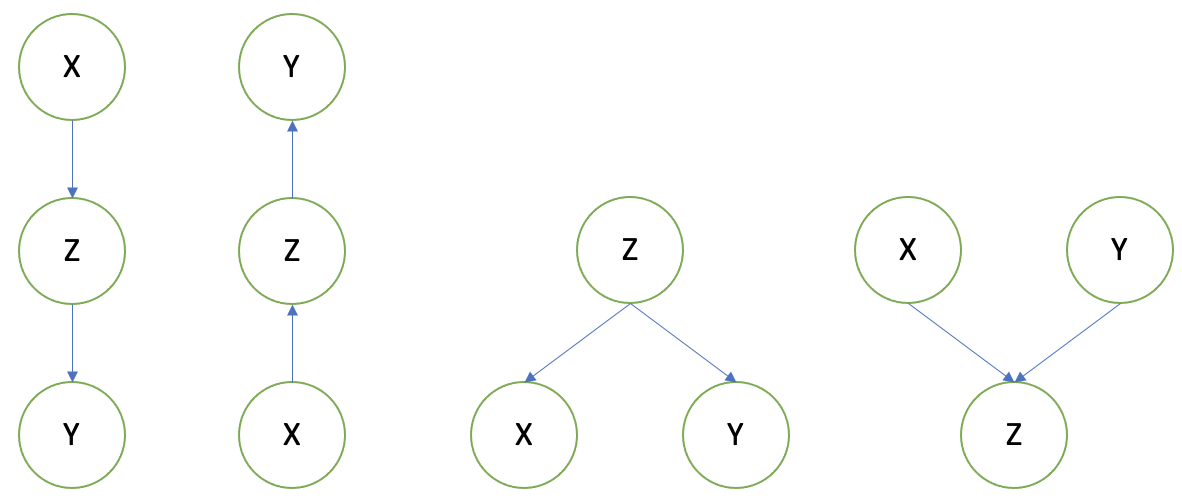
\includegraphics[width=0.6\textwidth]{images/graphical models/d-sep/d-sep-simple.png}
    \caption{Four patterns}
    \label{fig:d-sep-simple}
\end{figure}

\subsection*{Indirect Causal Effect $X\rightarrow Z\rightarrow Y$} 

Cause $X$ cannot influence effect $Y$ if $Z$ is observed, i.e.,  observed $Z$ blocks the influence of $X$ over $Y$. For the running example, as shown in Figure~\ref{fig:indirect-causal}, 


\begin{figure}[!htbp]
    \centering
    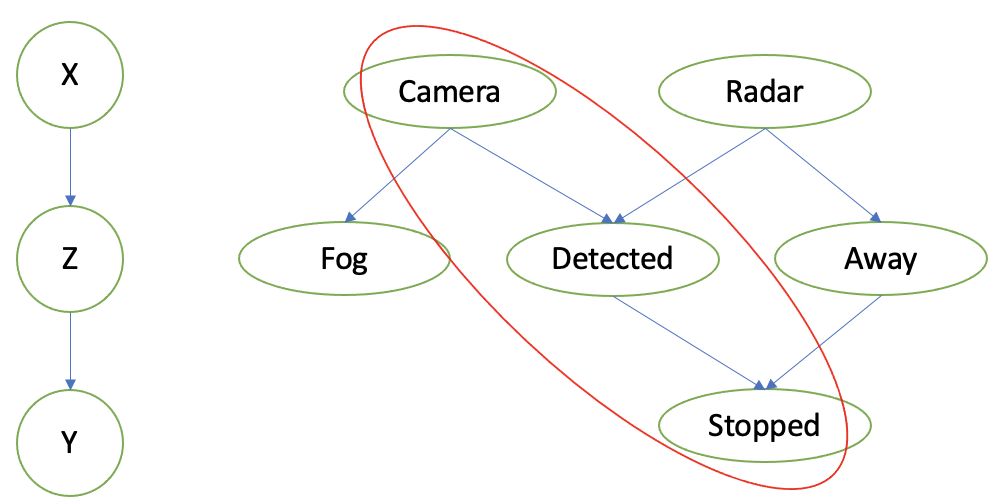
\includegraphics[width=0.5\textwidth]{images/graphical models/d-sep/indirect-causal.png}
    \caption{Indirect Causal Effect}
    \label{fig:indirect-causal}
\end{figure}

\subsection*{Indirect Evidential Effect $Y\rightarrow Z\rightarrow X$} Similarly, evidence $X$ cannot influence the cause $Y$ if $Z$ is observed. 


\subsection*{Common Cause $X\leftarrow Z\rightarrow Y$}

Once $Z$ is observed, one of the effects cannot influence the other.  Figure~\ref{fig:common-cause} presents a case of common cause in our running example. 

\begin{figure}[!htbp]
    \centering
    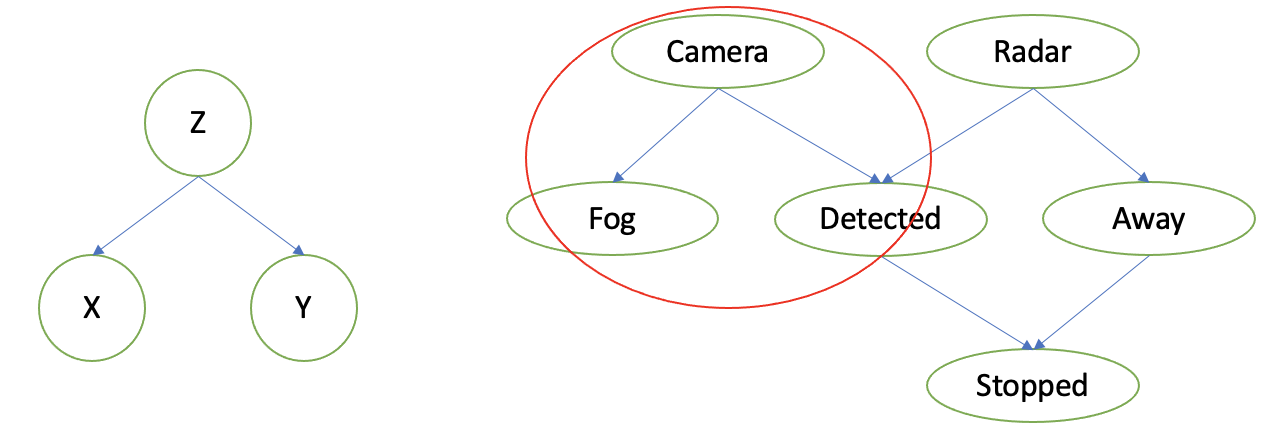
\includegraphics[width=0.6\textwidth]{images/graphical models/d-sep/common-cause.png}
    \caption{Common Cause}
    \label{fig:common-cause}
\end{figure}

\subsection*{Common Effect $X\rightarrow Z\leftarrow Y$} 

Unlike the above three cases where observing the middle variable $Z$ blocks the influence, the case of common effect is on the opposite, i.e., the influence is blocked when the common effect  $Z$  and its descendants are not observed. Figure~\ref{fig:common-effect} presents a case of common effect in our running example. 

\begin{figure}[!htbp]
    \centering
    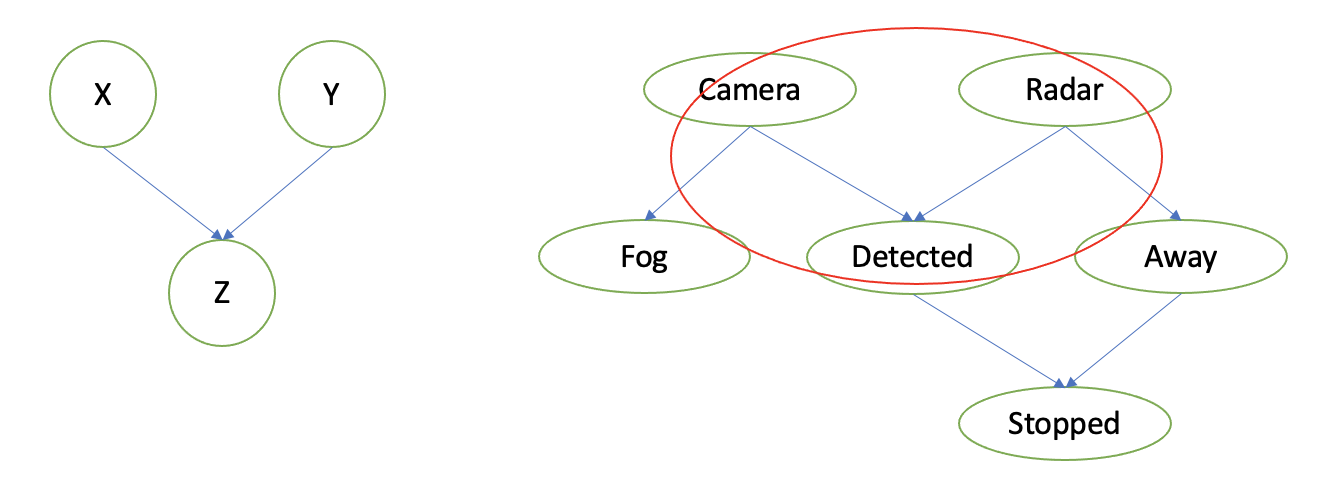
\includegraphics[width=0.6\textwidth]{images/graphical models/d-sep/common-effect.png}
    \caption{Common Effect}
    \label{fig:common-effect}
\end{figure}

\subsection{General Case: Active Trail and D-Separation}

Summarising the above discussion on local canonical cases (or v-structures), we have that 
\begin{itemize}
    \item Causal trail, $X\rightarrow Z\rightarrow Y$, is active if and only if $Z$ is not observed.  
    \item Evidential trail, $X\leftarrow Z\leftarrow Y$, is active if and only if  $Z$ is not observed. 
    \item Common cause, $X\leftarrow Z\rightarrow Y$, is active if and only if $Z$ is not observed. 
    \item Common effect, $X\rightarrow Z\leftarrow Y$, is active if and only if either $Z$ or one of its descendants is observed. 
\end{itemize}
%
Now we can consider the general case of $\dsep_G(X\bot Y|Z)$, where $X$, $Y$ and $Z$ may not be connected to each other. Actually, the graph can be large and the variables may be far away from each other. Fortunately, as we will introduce below, any complex case can be broken into repetitions of the local canonical cases. 

The D-separation algorithm is given in Algorithm~\ref{alg:dsepalg}. It collects all paths between $X$ and $Y$, without considering the directions of the edges. Then, as long as no paths are active given the observations $\{Z_1,...,Z_k\}$, the two variables $X$ and $Y$ are conditionally independent. 

\begin{algorithm}[!htbp]
\SetAlgoLined
%\KwResult{$S^0_i$ is the spike trains of input $X^0_i$}
\SetKwFunction{ConstructSubTree}{a set of training instances $D$}
$Path = $ all (undirected) paths from $X$ to $Y$ \\
\For{$path$ in $Path$}{
\eIf{isActive($path$, \{Z_1,...,Z_k\}) 
}{
\Return  $X\not\bot Y|\{Z_1,...,Z_k\}$
}
}
\Return $X\bot Y|\{Z_1,...,Z_k\}$
\caption{$\functionname{d-sep}_G$($X,Y,\{Z_1,...,Z_k\}$), where $X,Y,Z_i$ are nodes on a graph $G$}
 \label{alg:dsepalg}
\end{algorithm}

Now, we need to determine whether a path is active or not, i.e.,  $\functionname{isActive}($path$, \{Z_1,...,Z_k\})$, which can be done with Algorithm~\ref{alg:dsepalgactivetrail}. Simply speaking, it requires all local triplets on the path to be inactive to make the path inactive. 

\begin{algorithm}[!htbp]
\SetAlgoLined
%\KwResult{$S^0_i$ is the spike trains of input $X^0_i$}
\SetKwFunction{ConstructSubTree}{a set of training instances $D$}
Let $path = X_1,...,X_k$ \\
\For{all triplets $X_{i-1},X_{i},X_{i+1}$ on $path$}{
\eIf{$(X_{i-1},X_{i},X_{i+1})$ is inactive}{
\Return False
}
}
\Return True
\caption{$\functionname{isActive}$($path,\{Z_1,...,Z_k\}$), where $path$ is a path on the graph and $Z_i$ are nodes on $G$}
 \label{alg:dsepalgactivetrail}
\end{algorithm}

\subsection*{I-equivalence} 

Conditional independence assertions can be the same with different graphical structures, and I-equivalence is to capture such equivalence relation. 

\begin{definition}
Two graphs $G_1$ and $G_2$ are I-equivalent if $I(G_1)=I(G_2)$.
\end{definition} 

Let skeleton of a graph G be an undirected graph with an edge for every edge in $G$. We have that, if two graphs have the same set of skeletons and v-structures then they are I-equivalent.  



%\newpage
\section{Structure Learning}

There are mainly two approaches to acquire a graphical model. The first is through knowledge engineering, where the graphical model is constructed by hand with expert’s help. The second is through machine learning, by which  the graphical model is learned from a set of instances. 

First of all, the following is the problem statement for structure learning: 
\begin{tcolorbox}
Assume dataset $D$ is generated i.i.d. from distribution $P^*(X)$, and $P^*(X)$ is induced by an underlying graph $G^*$. The goal is to construct a graphical model $G$ such that it is as close as possible to $G^*$. 
\end{tcolorbox}

Considering that there may be many I-maps for $P^*$ and we cannot distinguish them from $D$, we know that $G^*$ is not identifiable. Nevertheless, in most cases, it is sufficient to recover $G^*$'s equivalence class. 

\subsection{Criteria of Structure Learning}

While our goal is to recover $G^*$'s equivalence class, this goal is nontrivial. One of the key issues is that the data instances sampled from the distribution $P^*(X)$ may be noisy. Therefore, we need to make decisions about including edges we are less sure about. Actually, too few edges means the possibility of missing out on dependencies, and too many edges means the possibility of spurious dependencies. 

\begin{example}
In a coin tossing example, we have two coins $X$ and $Y$, who are tossed independently. Assume that they are tossed 100 times, with the statistics shown in Table~\ref{tab:cointossingstructurallearning}. 
Are $X$ and $Y$ independent? 
\begin{table}[!htbp]
    \centering
    \begin{tabular}{|c|c|c|}
    \hline
    $X$ & $Y$ & times \\
    \hline
    head  & head & 27 \\
    head  & tail & 22 \\
    tail  & head & 25 \\
    tail  & head & 26 \\
    \hline
    \end{tabular}
    \caption{A simple coin tossing example}
    \label{tab:cointossingstructurallearning}
\end{table}
Actually, if we follow the exact computation, they are dependent. But we suspect that they should be independent, because the probability of getting exactly 25 in each category is small (approx. 1 in 1,000). 
\end{example}

Actually, in a conditional probability table, the number of entries grows exponentially with the of parent nodes. Therefore, the cost of adding a parent node can be very large. According to this, it is better to obtain a sparser, simpler structure.  
Actually, we can sometimes learn a better model by learning a model with fewer edges even if it does not represent the true distribution.

\subsection{Overview of Structure Learning Algorithms}

Basically, there are two classes of structural learning algorithms: 
\begin{itemize}
\item Constraint-based algorithms
\item Score-based algorithms 
\end{itemize}

Constraint-based algorithms are to find a graphical model whose implied independence constraints match those found in the data. On the other hand, score-based algorithms are to find a graphical model that can represent distributions that match the data (i.e., could have generated the data).

In the following, we introduce two 
%elements 
different directions of structural learning, by  the consideration of learning local relations and global structure, respectively. 

\subsection*{Local: Independence Tests}

For testing the independence between variables, we need measures of ``deviance-from-independence'' and rules  for accepting/rejecting hypothesis of independence. 
%
For the measures, we may consider e.g., mutual Information (K-L divergence) between joint and product of marginals, by having 
\begin{equation}\label{equ:miedges}
    d_I(D) = \frac{1}{|D|}\sum_{x_i,x_j}P(x_i,x_j)\log \frac{P(x_i,x_j)}{P(x_i)P(x_j)}
\end{equation}
for any two variables $X_i$ and $X_j$. 
Theoretically, $d_I(D)=0$ if $X_i$ and $X_j$ are independent, and $d_I(D)>0$ otherwise. In addition to $d_I(D)$, there may be other means to define the measures, such as Pearson’s Chi-squared test.  

Based on the measure,  we can define the acceptance rule as
\begin{equation}
    R_{d,t}(D)=
    \begin{cases}
    \text{Accept} & d(D) \leq t \\
    \text{Reject} & d(D) > t \\
    \end{cases}
\end{equation}
where $t$ is a pre-specified threshold. We remark that false rejection probability due to choice of $t$ is its $p$-value (refer to hypothesis testing). Alternatively, we may take Chow-Liu algorithm to construct a tree-like graphical model as follows: 
\begin{enumerate}
    \item find maximum weight spanning tree based on the values we compute in Equation (\ref{equ:miedges}); there are existing algorithms for this purpose, such as the Kruskal’s algorithm and the Prim’s algorithm. 
    \item pick a root node and assign edge directions.  
\end{enumerate}

\subsection*{Global: Structure Scoring}

Similarly as the local case, we need measures to evaluate the goodness of a graphical model and rules for accepting/rejecting hypothesis of goodness. 
%
There are different ways to define measures, including 
\begin{itemize}
    \item Log-likelihood Score for G with $n$ variables 
\begin{equation}
    Score_L(G,D) = \sum_{D}\sum_{i=1}^n \log P(x_i|pa(x_i))
\end{equation}
which can be seen as the loss of using graph $G$ to predict $D$. 
    \item Bayesian Score 
\begin{equation}
    Score_B(G,D) = \log P(D|G) + \log P(G)
\end{equation}
which, in addition to the log-likelihood score $\log P(D|G)$, it also consider the prior $P(G)$. 
    \item Bayes score with penalty term 
\begin{equation}
    Score_{BIC}(G,D) = L(G, D)- \frac{\log |D|}{2}||G||
\end{equation}
where $L(G, D)$ is the loss of using $G$ to predict $D$, and  $||G||$ is the complexity of the graph $G$. 
\end{itemize}


%\subsection*{Model Search}

Once defined the scores, the structure learning is to search for a graphical structure with the highest score. It is known that finding the optimal one among those structures with at most $k$ parents is NP-hard for $k>1$. To deal with the high complexity, there are multiple methods including e.g., 
\begin{itemize}
    \item Greedy search 
    \item Greedy search with restarts
    \item MCMC methods
\end{itemize}
For the greedy search, it repeatedly does the following: 
\begin{enumerate}
    \item score all possible single changes, and
    \item select the best change to apply if there are any changes that lead to better performance than the existing structure.
\end{enumerate}  


\subsection{Practice}

The following code uses the \textbf{pomegranate} package to automatically learn structures from a simple dataset. 

\begin{lstlisting}[language=Python]
from pomegranate import BayesianNetwork
import seaborn, time, numpy, matplotlib
seaborn.set_style('whitegrid')

import pandas as pd
X = pd.DataFrame({'1':[0,0,0,1,0], '2':[0,0,1,0,0], '3':[1,1,0,0,1], '4':[0,1,0,1,1]})
X = X.to_numpy()

tic = time.time()
model = BayesianNetwork.from_samples(X) 
t = time.time() - tic
p = model.log_probability(X).sum()
print("Greedy")
print("Time (s): ", t)
print("P(D|M): ", p)
model.plot()

tic = time.time()
model = BayesianNetwork.from_samples(X, algorithm='exact-dp') 
t = time.time() - tic
p = model.log_probability(X).sum()
print("exact-dp")
print("Time (s): ", t)
print("P(D|M): ", p)
model.plot()

tic = time.time()
model = BayesianNetwork.from_samples(X, algorithm='exact') 
t = time.time() - tic
p = model.log_probability(X).sum()
print("exact")
print("Time (s): ", t)
print("P(D|M): ", p)
model.plot()
\end{lstlisting}

\notincludedinbook{
\newpage
\chapter{Sensitivity Analysis}

As suggested earlier, it is possible that some probability tables of a graphical model can be obtained through machine learning. However, considering that a machine learning may be subject to various safety risks, it is useful to study how such safety risks on machine learning learning may affect the inference on the graphical model. In particular, we consider the following problem: 

\begin{tcolorbox}
 Given a certain constraint on the perturbations and an MAP query, it is to determine whether or not the perturbed values may lead to a different decision about the MAP query.
\end{tcolorbox}

The following is an example from \cite{NIPS2014_09662890}. 

\begin{example}
Consider a simple two-node graphical model $G=(\{X_1,X_2\}, \{X_1 \rightarrow X_2\}, P)$, where $P(X_1=1)=0.45$ and $P(X_2=1|X_1=1)=0.2$ and $P(X_2=1|X_1=0)=0.9$. We have that 
\begin{equation}
MAP(G) = (X_1=1, X_2=0)
\end{equation}

Now, if consider the following perturbation constraint
\begin{equation}
    |P(X_1=1)-0.45| \leq 0.06
\end{equation}
does the assignment $(X_1=1, X_2=0)$ continue to be the $MAP(G)$? 
\end{example}



}


\noexercises{
\newpage
\Extrachap{Exercise} 

\begin{question}
Try to explain another inter-causal reasoning in Figure~\ref{fig:cameratables}, over the three variables $Detected$, $Stopped$, and $Away$. 
\end{question}


\begin{question}
Implement the Chow-Liu algorithm for the \textbf{iris} dataset.  
\end{question}


\begin{question}
Can you propose a solution for the sensitivity analysis?   
\end{question}
}


\chapter{Competition: Resilience to Adversarial Attack}\label{sec:competitionresilience}

This is a student competition to address two key issues in modern deep learning, i.e., 
\begin{itemize}
    \item[O1] how to find better adversarial attacks, and
    \item[O2] how to train a deep learning model with better robustness to the adversarial attacks.
\end{itemize}
We provide a template code (\textbf{Competition/Competition.py}), where there are two code blocks corresponding to the training and the attack, respectively. The two code blocks are filled with the simplest implementations representing the baseline methods, and the participators are expected to replace the baseline methods with their own implementations, in order to achieve better performance regarding the above O1 and O2. 

\section{Submissions}

In the end, we will collect submissions from the students and rank them according to a pre-specified metric taking into consideration both O1 and O2. 
%
Assume that we have $n$ students participating in this competition, and we have a set $S$ of submissions.

\vspace{1em}
\begin{tcolorbox}
Every student with student number $i$ will submit a  package \textbf{$i$.zip},  which includes two files:
\begin{enumerate}
    \item $i$\textbf{.pt}, which is the file to save the trained model, and
    \item competition\_$i$\textbf{.py}, which is your  script after updating the two code blocks in \textbf{Competition.py} with your implementations.  
\end{enumerate}  \\NB: Please carefully follow the naming convention as indicated above, and we will not accept submissions which do not follow the naming convention. 
\end{tcolorbox}


\section{Source Code}

The template source code of the competition is available at 
\begin{tcolorbox}[center, boxsep=0pt, left=1ex, right=1ex, width = 9cm, before upper=\strut, tcbox width = minimum center, box align=center, halign=center, colback=white, colframe=blue!50!black]
\url{https://github.com/xiaoweih/AISafetyLectureNotes/tree/main/Competition}
\end{tcolorbox}


\vspace{2em}

In the following, we will explain each part of the code. 



\subsection*{Load packages}

First of all, the following code piece imports a few packages that are needed. 

\begin{lstlisting}[language=Python]
import numpy as np
import pandas as pd
import torch
import torch.nn as nn
import torch.nn.functional as F
from torch.utils.data import Dataset, DataLoader
import torch.optim as optim
import torchvision
from torchvision import transforms
from torch.autograd import Variable
import argparse
import time
import copy
\end{lstlisting}

Note: You can add necessary packages for your implementation. 



\subsection*{Define competition ID} The below line of code defines the student number. By replacing it with your own student number, it will automatically output the file $i$\textbf{.pt} once you trained a model. 

%You need to change the below id into your student ID number. This will ensure that the saved model (to be explained later) is named as $i$\textbf{.pt} automatically. 


\begin{lstlisting}[language=Python]
# input id
id_ = 1000
\end{lstlisting}


\subsection*{Set training parameters}

The following is to set the hyper-parameters for training. It considers e.g., batch size, number of epochs, whether to use CUDA, learning rate, and random seed. You may change them if needed. 

\begin{lstlisting}[language=Python]
# setup training parameters
parser = argparse.ArgumentParser(description='PyTorch MNIST Training')
parser.add_argument('--batch-size', type=int, default=128, metavar='N',
                    help='input batch size for training (default: 128)')
parser.add_argument('--test-batch-size', type=int, default=128, metavar='N',
                    help='input batch size for testing (default: 128)')
parser.add_argument('--epochs', type=int, default=10, metavar='N',
                    help='number of epochs to train')
parser.add_argument('--lr', type=float, default=0.01, metavar='LR',
                    help='learning rate')
parser.add_argument('--no-cuda', action='store_true', default=False,
                    help='disables CUDA training')
parser.add_argument('--seed', type=int, default=1, metavar='S',
                    help='random seed (default: 1)')
args = parser.parse_args(args=[]) 
\end{lstlisting}

\subsection*{Toggle GPU/CPU}

Depending on whether you have GPU in your computer, you may toggle between devices with the below code. Just to remark that, for this competition, the usual CPU is sufficient and a GPU is not needed. 

\begin{lstlisting}[language=Python]
# judge cuda is available or not
use_cuda = not args.no_cuda and torch.cuda.is_available()
#device = torch.device("cuda" if use_cuda else "cpu")
device = torch.device("cpu")

torch.manual_seed(args.seed)
kwargs = {'num_workers': 1, 'pin_memory': True} if use_cuda else {}
\end{lstlisting}


\subsection*{Loading dataset and define network structure}

In this competition, we use the same dataset (FashionMNIST) and the same network architecture. The following code specify how to load dataset and how to construct a 3-layer neural network. Please do not change this part of code. 

\begin{lstlisting}[language=Python]
####################################################don't change the below code    ####################################################

train_set = torchvision.datasets.FashionMNIST(root='data', train=True, download=True, transform=transforms.Compose([transforms.ToTensor()]))
train_loader = DataLoader(train_set, batch_size=args.batch_size, shuffle=True)

test_set = torchvision.datasets.FashionMNIST(root='data', train=False, download=True, transform=transforms.Compose([transforms.ToTensor()]))
test_loader = DataLoader(test_set, batch_size=args.batch_size, shuffle=True)

# define fully connected network
class Net(nn.Module):
    def __init__(self):
        super(Net, self).__init__()
        self.fc1 = nn.Linear(28*28, 128)
        self.fc2 = nn.Linear(128, 64)
        self.fc3 = nn.Linear(64, 32)
        self.fc4 = nn.Linear(32, 10)

    def forward(self, x):
        x = self.fc1(x)
        x = F.relu(x)
        x = self.fc2(x)
        x = F.relu(x)
        x = self.fc3(x)
        x = F.relu(x)
        x = self.fc4(x)
        output = F.log_softmax(x, dim=1)
        return output

####################################################end of "don't change the below code"   ####################################################
\end{lstlisting}


\subsection*{Adversarial Attack}

The part is the place needing your implementation, for O1. In the template code, it includes a baseline method which uses random sampling to find adversarial attacks. You can only replace the  middle part of the function with your own implementation (as indicated in the code), and are not allowed to change others. 

\begin{lstlisting}[language=Python]
'generate adversarial data, you can define your adversarial method'
def adv_attack(model, X, y, device):
    X_adv = Variable(X.data)
    
    ############################################Note: below is the place you need to edit to implement your own attack algorithm
    ############################################
    
    random_noise = torch.FloatTensor(*X_adv.shape).uniform_(-0.1, 0.1).to(device)
    X_adv = Variable(X_adv.data + random_noise)
    
    ############################################ end of attack method
    ############################################
    
    return X_adv
\end{lstlisting}


\subsection*{Evaluation Functions}

Below are two supplementary functions that return loss and accuracy over test dataset and adversarially attacked test dataset, respectively. We note that the function \textbf{adv\_attack} is used in the second function. You are not allowed to change these two functions. 

\begin{lstlisting}[language=Python]
'predict function'
def eval_test(model, device, test_loader):
    model.eval()
    test_loss = 0
    correct = 0
    with torch.no_grad():
        for data, target in test_loader:
            data, target = data.to(device), target.to(device)
            data = data.view(data.size(0),28*28)
            output = model(data)
            test_loss += F.nll_loss(output, target, size_average=False).item()
            pred = output.max(1, keepdim=True)[1]
            correct += pred.eq(target.view_as(pred)).sum().item()
    test_loss /= len(test_loader.dataset)
    test_accuracy = correct / len(test_loader.dataset)
    return test_loss, test_accuracy

def eval_adv_test(model, device, test_loader):
    model.eval()
    test_loss = 0
    correct = 0
    with torch.no_grad():
        for data, target in test_loader:
            data, target = data.to(device), target.to(device)
            data = data.view(data.size(0),28*28)
            adv_data = adv_attack(model, data, target, device=device)
            output = model(adv_data)
            test_loss += F.nll_loss(output, target, size_average=False).item()
            pred = output.max(1, keepdim=True)[1]
            correct += pred.eq(target.view_as(pred)).sum().item()
    test_loss /= len(test_loader.dataset)
    test_accuracy = correct / len(test_loader.dataset)
    return test_loss, test_accuracy
\end{lstlisting}


\subsection*{Adversarial Training}

Below is the second place needing your implementation, for O2. In the template code, there is a baseline method. You can replace relevant part of the code as indicated in the code. 

\begin{lstlisting}[language=Python]
#train function, you can use adversarial training
def train(args, model, device, train_loader, optimizer, epoch):
    model.train()
    for batch_idx, (data, target) in enumerate(train_loader):
        data, target = data.to(device), target.to(device)
        data = data.view(data.size(0),28*28)
        
        #use adverserial data to train the defense model
        #adv_data = adv_attack(model, data, target, device=device)
        
        #clear gradients
        optimizer.zero_grad()
        
        #compute loss
        #loss = F.nll_loss(model(adv_data), target)
        loss = F.nll_loss(model(data), target)
        
        #get gradients and update
        loss.backward()
        optimizer.step()
        
#main function, train the dataset and print train loss, test loss for each epoch
def train_model():
    model = Net().to(device)
    
    #####################################################################
    ## Note: below is the place you need to edit to implement your own training algorithm
    ##       You can also edit the functions such as train(...). 
    #####################################################################
    
    optimizer = optim.SGD(model.parameters(), lr=args.lr)
    for epoch in range(1, args.epochs + 1):
        start_time = time.time()
        
        #training
        train(args, model, device, train_loader, optimizer, epoch)
        
        #get trnloss and testloss
        trnloss, trnacc = eval_test(model, device, train_loader)
        advloss, advacc = eval_adv_test(model, device, train_loader)
        
        #print trnloss and testloss
        print('Epoch '+str(epoch)+': '+str(int(time.time()-start_time))+'s', end=', ')
        print('trn_loss: {:.4f}, trn_acc: {:.2f}%'.format(trnloss, 100. * trnacc), end=', ')
        print('adv_loss: {:.4f}, adv_acc: {:.2f}%'.format(advloss, 100. * advacc))
        
    adv_tstloss, adv_tstacc = eval_adv_test(model, device, test_loader)
    print('Your estimated attack ability, by applying your attack method on your own trained model, is: {:.4f}'.format(1/adv_tstacc))
    print('Your estimated defence ability, by evaluating your own defence model over your attack, is: {:.4f}'.format(adv_tstacc))
    ############################################
    ## end of training method
    ############################################
    
    #save the model
    torch.save(model.state_dict(), str(id_)+'.pt')
    return model
\end{lstlisting}


\subsection*{Define Distance Metrics}

In this competition, we take the $L_\infty$ as the distance measure. You are not allowed to change the code. 

\begin{lstlisting}[language=Python]
#compute perturbation distance
def p_distance(model, train_loader, device):
    p = []
    for batch_idx, (data, target) in enumerate(train_loader):
        data, target = data.to(device), target.to(device)
        data = data.view(data.size(0),28*28)
        data_ = copy.deepcopy(data.data)
        adv_data = adv_attack(model, data, target, device=device)
        p.append(torch.norm(data_-adv_data, float('inf')))
    print('epsilon p: ',max(p))
\end{lstlisting}

\subsection*{Supplementary Code for Test Purpose}

In addition to the above code, we also provide two lines of code for testing purpose. You must comment them out in your submission. 
%
The first line is to call the \textbf{train\_model()} method to train a new model, and the second is to check the quality of attack based on a model. 

\begin{lstlisting}[language=Python]
#Comment out the following command when you do not want to re-train the model
#In that case, it will load a pre-trained model you saved in train_model()
model = train_model()

#Call adv_attack() method on a pre-trained model
#The robustness of the model is evaluated against the infinite-norm distance measure
#!!! Important: MAKE SURE the infinite-norm distance (epsilon p) less than 0.11 !!!
p_distance(model, train_loader, device)
\end{lstlisting}

\section{Implementation Actions}

Below, we summarise the actions that need to be taken for the completion of a submission: 

\begin{enumerate}
    \item You must assign the variable \textbf{id\_} with your student ID $i$;
    \item You need to update the \textbf{adv\_attack} function with your adversarial attack method; 
    \item You may change the hyper-parameters defined in \textbf{parser} if needed; 
    \item You must make sure the perturbation distance less than \textbf{0.11}, (which can be computed by \textbf{p\_distance} function); 
    \item You need to update the \textbf{train\_model} function (and some other functions that it called such as \textbf{train}) with your own training method;
    \item You need to use the line ``model = train\_model()'' to train a model and check whether there is a file $i$\textbf{.pt}, which stores the weights of your trained model;
    \item You must submit $i$\textbf{.zip}, which includes two files $i$\textbf{.pt} (saved model) and competition\_$i$\textbf{.py} (your script). 
\end{enumerate}

%You can use the following script to train the defense model, \textbf{note that}  2. you caan use the model, data, target to define your adversarial method from line 106, don't modify the line 105; 3. you also can modify hyper-parameters, e.g., epochs, learning rate, etc, or use special regularizers; 4. you can save the defense model through the function in line 185; 5. do not modify the net architecture; 6. you can test the script from line 190, and you need to annotate the test code in the submission file; 7. you can use adversarial data to train through line 125; 8. you need to submit $i$\textbf{.zip}, which includes two files $i$\textbf{.pt} (saved model) and competition\_$i$\textbf{.py} (your script).       




\iffalse
\begin{enumerate}
\item Train and test the net.

%The following is the way how to call this functionality: 
%\begin{cmds}
%python3 i/aisafetysubmission.py --training --dataset 'data' --model '[path-to-saved-model]/i.pt'
%\end{cmds}
%Note that, we require the saved model has $i$ as its name. This is to make sure that there won't be any clash between submissions. The expected output should include the following statement: 
%\begin{cmds}
%The model is saved as '[path-to-saved-model]/i.pt' for the dataset 'data'
%\end{cmds}
    \item Attack function
    \begin{itemize}
        \item \textbf{input}: a saved model $M_i$, an index number $k\in \{0..9000\}$, a number $m\in\{100...1000\}$
        \item \textbf{output}: $m$ adversarial examples as in a set $Adv_i = (\textbf{X}_{adv},\textbf{y}_{adv})$, and their average perturbations $p_i$ over $L_\infty$ norm distance
        \item \textbf{additional description}: the attacked data instances are indexed from $k$ to $k+m-1$ in the test dataset, such that one adversarial example is generated for every data instance. \xiaowei{We may need to specify the format of the adversarial examples $(\textbf{X}_{adv},\textbf{y}_{adv})$.}
    \end{itemize}
The following is the way how to call this functionality: 
\begin{cmds}
python3 i/aisafetysubmission.py --attack --dataset 'data' --model '[path-to-saved-model]/i.pt' --startingIndex [index-of-test-dataset] --number [number-of-adversarial-examples] --adversary '[path-to-adversarial-examples]/i/'
\end{cmds}
Note that, after [path-to-adversarial-examples] we have a sub-folder $/i/$. This is to make sure that  there won't be any clash between submissions. The expected output should include the following statement: 
\begin{cmds}
The adversarial examples are stored in '[path-to-adversarial-examples]/i/' for the dataset 'data'. They are generated by attacking [number-of-adversarial-examples] data instances in the test dataset, starting from index [index-of-test-dataset]. The average L_inf perturbation is [returned_average_perturbation]
\end{cmds}
    \item Evaluation function
    \begin{itemize}
        \item \textbf{input}: a saved model $M_i$, a set $Adv_j$ of adversarial examples, where $j\in S$
        \item \textbf{output}: the score $s_{i,j}$, representing the accuracy of $M_i$ over the union of $Adv_j=(\textbf{X}_{adv},\textbf{y}_{adv})$ and test dataset $(\textbf{X}_{test},\textbf{y}_{test})$. 
    \end{itemize}
The following is the way how to call this functionality. Note that, while $j$ could be any number in $S$ so that your model can run through other submissions, you can use $j=i$ to test whether your command work or not.  
\begin{cmds}
python3 i/aisafetysubmission.py --evaluation --dataset 'data' --model '[path-to-saved-model]/i.pt' --adversary '[path-to-adversarial-examples]/j/'
\end{cmds}
\end{enumerate}
The expected output should include the following statement: 
\begin{cmds}
The score of evaluating those adversarial examples in '[path-to-adversarial-examples]/j/' is [returned_accuracy]
\end{cmds}

\fi

\iffalse

\section{Submission Files} 

You are expected to submit the following two files:  
\begin{itemize}
    \item \textbf{$i$.zip} 
    \item \textbf{$i$.pt}
\end{itemize}
Note that, please make sure that \textbf{$i$.pt} is the one generated by the first command.  

\fi

\subsection*{Sanity Check} 

Please make sure that the following constraints are satisfied. Your submission won't be marked if they are not followed. 

\begin{itemize}
    \item Submission file: please follow the naming convention as suggested above. 
    \item Make sure your code can run smoothly. 
    \item Comment out the two lines ``model = train\_model()'' and ``p\_distance(model, train\_loader , device)'', which are for test purpose. 
    %\item '[path-to-saved-model]/i.h5' and '[path-to-adversarial-examples]/j/': please follow the naming convention as suggested above
    %\item make sure your output on the screen is the same as we suggested above. 
    %\item The generation of 100 adversarial examples won't take more than 5 minutes; that is, if we ask for 300 adversarial examples, it won't take more than 15 minutes. 
\end{itemize}



\section{Evaluation Criteria}

Assume that, among the submissions $S$, we have $n$ submissions that can run smoothly and correctly. We can get model $M_i$ by reading the file \textbf{$i$.pt}. 
%In addition, for each 

Then, we collect the following 
%two statistics: 
%\begin{equation}
%    \textbf{P}=(p_1,...,p_n)
%\end{equation}
%for the average perturbation and 
matrix 
\begin{equation}
\textbf{Score} = ~~~
\begin{blockarray}{cccccc}
\begin{block}{l(ccccc)}
  \textbf{i=1} & s_{11} & s_{12} &  ... & s_{1(n-1)} & s_{1n}  \\
  \textbf{i=2} & s_{21} & s_{22} & ... & s_{2(n-1)} & s_{2n}  \\
  ... \\
  \textbf{i=n-1} & s_{(n-1)1} & s_{(n-1)2} & ... & s_{(n-1)(n-1)} & s_{(n-1)n}  \\
  \textbf{i=n} & s_{n1} & s_{n2} & ... & s_{n(n-1)} & s_{nn}  \\
\end{block}
& \textbf{j=1} & \textbf{j=2} & ... & \textbf{j=n-1} & \textbf{j=n}  \\
\end{blockarray}
\label{equ:evaluationscores}
\end{equation}
for the mutual evaluation scores of using $M_i$ to evaluate $Atk_j$ (defined in function \textbf{adv\_attack}). The score $s_{ij}$ is the \textbf{test accuracy} obtained by using \textbf{adv\_attack} function from the file competition~\_$j$\textbf{.py} to attack the model from \textbf{$i$.pt}. From Equation (\ref{equ:evaluationscores}), we get $j$'s attacking ability by letting 
\begin{equation}
    AttackAbility_j = \sum_{i=1}^n \textbf{Score}_{i,j}
\end{equation}
to be the total of the scores of $j$-th column. Let $\textbf{AttackAbility}$ be the vector of $AttackAbility_j$. Moreover, we get $i$'s defence ability by letting 
\begin{equation}
    DefenceAbility_i = \sum_{j=1}^n \textbf{Score}_{i,j},
\end{equation} 
Let $\textbf{DefenceAbility}$ be the vector of $DefenceAbility_i$.
Then, for the vectors %$\textbf{P}$,
$\textbf{AttackAbility}$ and $\textbf{DefenceAbility}$, we apply Softmax function to normalise to get 
\begin{equation}
    %\sigma(\frac{1}{\textbf{P}}),
    \sigma(\frac{1}{\textbf{AttackAbility}}), \sigma(\textbf{DefenceAbility})
\end{equation}
Then, the final score for the submission $i$ is 
\begin{equation}
    FinalScore_i = \sigma(
    %\sigma(\frac{1}{\textbf{P}})+
    \sigma(\frac{1}{\textbf{AttackAbility}})+\sigma(\textbf{DefenceAbility}))_i
\end{equation}

Note that, to reduce the impact of randomness,
%on selecting the $m$ test data instances, 
we may conduct 3 rounds of the above process to get the average $FinalScore_i$ for every submission. 


\section{Q\&A} 

\subsection*{Will the running time, memory, and CPU usage be considered in marking for the training and attack?}

We only evaluate against a trained model, so no consideration will be given on the running time, memory, and CPU usage in training. For the attack, it will run on marker's computer, so we expect it to run in a reasonable time, e.g., within 1 min for a single image. 

\subsection*{Can we use external pip packages for purposes like hyperparameter tuning? }

You can use external libraries as long as they are consistent with the libraries we suggested for this module, and can be installed easily through either pip or annaconda. 

You can also use package for e.g., attack, but you have to make sure that the package will run well in normal circumstance (so that the markers can run the package). 

\subsection*{Would it be OK to search for popular algorithm and then try to fix that to my submission?}

Yes, you can. Actually, you are free to take -- and adapt -- any existing algorithms/implementations – this is also a skill that is nowadays quite useful in ML field. This will probably be the case for most people.

\subsection*{How would you make sure the competition is fair? I am worrying about that some submissions may try to overfit the test dataset.}

The test dataset is not open, so nobody has access to the test dataset before competition. 



\subsection*{Architectural search was mentioned in today's Q\&A session, but I think it may be unhelpful since our target network architecture is fixed. The only thing I could come up with is to use Dropouts to deactivate some nodes to achieve a pseudo different net structure?}

Architecture search might not be the most suitable technique to consider here – I mentioned it simply because there was a question I was asked. 

\subsection*{Automated hyperparameter tunning was also mentioned in today's Q\&A. Also, you mentioned several sessions ago that we should make sure to use some widely used reliable libraries. Given that I am using ray tune currently, do you have any recommendations on this?}

It might be OK to try, if you want to exercise on hyper-parameter tuning. I do not have personal preference on the libraries, and you can select whichever you feel OK with. Just to remind you: for the submission, we only look at the trained weights, so will not be able to consider how you tune the parameters to get the weights. 

\subsection*{How will the score of attack/defense be measured? Do we use loss or accuracy or loss \& accuracy to evaluate the result?} 

Please refer to the $p\_distance$ function of the template code for a good understanding of this question.

\subsection*{How could you deal with the connection problem when downloading dataset through python IDLE?} 

Please use CMD (windows) or Terminal (mac) to download the dataset.



\iffalse
\subsection*{How about I didn't successfully implement all the three functionalities?}

The following are the marks for individual functionalities: 
\begin{itemize}
    \item Training: 20 marks 
    \item Attack: 20 marks
    \item Evaluation: 10 marks
\end{itemize}

You will get rewarded on the functionalities you 
completed. 

\subsection*{How about some of the functionalities are not implemented correctly?}

You will not participate in the competition and will only get the marks on those functionalities that you have correctly implemented. 

\fi